% !TEX TS-program = pdfLaTeX+MakeIndex+BibTeX
% !TEX encoding = UTF-8 Unicode

\PassOptionsToPackage{unicode}{hyperref}
\PassOptionsToPackage{naturalnames}{hyperref}

\documentclass[tg]{mdtufsm}

\usepackage[T1]{fontenc}
\usepackage{fix-cm}
\usepackage{times, color}
\usepackage[utf8]{inputenc}
\usepackage{graphicx}
\usepackage{amsmath,latexsym,amssymb}
%\usepackage[hidelinks]{hyperref}
\usepackage[hidelinks,
            bookmarksopen=true,linktoc=none,colorlinks=true,
            linkcolor=black,citecolor=black,filecolor=magenta,urlcolor=blue,
            pdftitle={Desenvolvimento e Reutilização de Testes Automatizados em Aplicações Web},
            pdfauthor={Lucas Antunes Amaral},
            pdfsubject={Trabalho de Graduação},
            pdfkeywords={Linguagens de Programação, Qualidade de Software, Testes de Software, Selinum HQ, Cucumber, Informática, UFSM}
            ]{hyperref}
%\usepackage[brazilian]{babel}

%\usepackage{fontspec}
%\setmainfont{Linux Libertine G}

%%% PAGE DIMENSIONS
\usepackage[inner=30mm,outer=20mm,top=30mm,bottom=20mm]{geometry}
\usepackage{epstopdf}
\usepackage{graphicx}
% \geometry{margin=2in} % for example, change the margins to 2 inches all round
% \geometry{landscape} % set up the page for landscape

% \usepackage[parfill]{parskip} % Activate to begin paragraphs with an empty line rather than an indent

%%% PACKAGES
%\usepackage{amsfonts}
%\usepackage{color}
%\usepackage{booktabs} % for much better looking tables
%\usepackage{array} % for better arrays (eg matrices) in maths
%\usepackage{paralist} % very flexible & customisable lists (eg. enumerate/itemize, etc.)
\usepackage{verbatim} % adds environment for commenting out blocks of text & for better verbatim
\usepackage{listings}
\usepackage{parcolumns}
%\usepackage{microtype}
%\usepackage[numbers]{natbib}
%\usepackage{subfig} % make it possible to include more than one captioned figure/table in a single float
% These packages are all incorporated in the memoir class to one degree or another...

\lstset{
	basicstyle=\scriptsize\ttfamily,
	tabsize=2,
	frame=single,
	breaklines=true,
	breakatwhitespace=true,
	xleftmargin=0cm,
	xrightmargin=0cm,
	literate=
		{á}{{\'a}}1 {é}{{\'e}}1 {í}{{\'i}}1 {ó}{{\'o}}1 {ú}{{\'u}}1
		{Á}{{\'A}}1 {É}{{\'E}}1 {Í}{{\'I}}1 {Ó}{{\'O}}1 {Ú}{{\'U}}1
		{à}{{\`a}}1 {è}{{\`e}}1 {ì}{{\`i}}1 {ò}{{\`o}}1 {ù}{{\`u}}1
		{À}{{\`A}}1 {È}{{\'E}}1 {Ì}{{\`I}}1 {Ò}{{\`O}}1 {Ù}{{\`U}}1
		{ä}{{\"a}}1 {ë}{{\"e}}1 {ï}{{\"i}}1 {ö}{{\"o}}1 {ü}{{\"u}}1
		{Ä}{{\"A}}1 {Ë}{{\"E}}1 {Ï}{{\"I}}1 {Ö}{{\"O}}1 {Ü}{{\"U}}1
		{â}{{\^a}}1 {ê}{{\^e}}1 {î}{{\^i}}1 {ô}{{\^o}}1 {û}{{\^u}}1
		{Â}{{\^A}}1 {Ê}{{\^E}}1 {Î}{{\^I}}1 {Ô}{{\^O}}1 {Û}{{\^U}}1
		{ã}{{\~a}}1 {Ã}{{\~A}}1
		{ç}{{\c c}}1 {Ç}{{\c C}}1
}

% For Computer Modern:
%\def\Cpp{{C\nolinebreak[4]\hspace{-.05em}\raisebox{.4ex}{\tiny\bf ++}}}
% For Linux Libertine G
\def\Cpp{{C\nolinebreak[4]\raisebox{.20ex}{\small\bf++}}}

\newcommand{\todo}[1]{\textsf{\color{red}#1}}

%%=============================================================================
%% Trampa para corrigir o bug do hyperref que redefine o caption das figuras e das
%% tabelas, não colocando o nome ``Figura'' antes do número do mesmo na lista
%%=============================================================================

\makeatletter

\long\def\@caption#1[#2]#3{%
  \expandafter\ifx\csname if@capstart\expandafter\endcsname
                  \csname iftrue\endcsname
    \global\let\@currentHref\hc@currentHref
  \else
    \hyper@makecurrent{\@captype}%
  \fi
  \@ifundefined{NR@gettitle}{%
    \def\@currentlabelname{#2}%
  }{%
    \NR@gettitle{#2}%
  }%
  \par\addcontentsline{\csname ext@#1\endcsname}{#1}{%
    \protect\numberline{\csname fnum@#1\endcsname ~-- }{\ignorespaces #2}%
  }%
  \begingroup
    \@parboxrestore
    \if@minipage
      \@setminipage
    \fi
    \normalsize
    \expandafter\ifx\csname if@capstart\expandafter\endcsname
                    \csname iftrue\endcsname
      \global\@capstartfalse
      \@makecaption{\csname fnum@#1\endcsname}{\ignorespaces#3}%
    \else
      \@makecaption{\csname fnum@#1\endcsname}{%
        \ignorespaces
        \ifHy@nesting
          \expandafter\hyper@@anchor\expandafter{\@currentHref}{#3}%
        \else
          \Hy@raisedlink{%
            \expandafter\hyper@@anchor\expandafter{%
              \@currentHref
            }{\relax}%
          }%
          #3%
        \fi
      }%
    \fi
    \par
  \endgroup
}

\makeatother

%%% END Article customizations

\title{Desenvolvimento e Reutilização de Testes Automatizados em Aplicações Web}
\author{Amaral}{Lucas Antunes}
\course{Curso de Ciência da Computação}
\altcourse{Curso de Ciência da Computação}
\institute{Centro de Tecnologia}
\degree{Bacharel em Ciência da Computação}

\trabalhoNumero{}
\advisor[Profª.]{Drª.}{Charão}{Andrea Schwertner}
\orientadoratrue

\committee[Profª. Dr.]{Bernardi}{Giliane}{UFSM}
\committee[MSc.]{Pereira}{Adriano}{UFSM}

\date{8}{Outubro}{2014}

\keyword{Qualidade de Software}
\keyword{Testes automatizados de Software}
\keyword{Linguagens de Programação}
\keyword{Selenium HQ}
\keyword{Cucumber}

%\date{} % Activate to display a given date or no date (if empty), otherwise the current date is printed

\begin{document}
\maketitle
\makeapprove

\begin{abstract}
A constante busca pela qualidade de uma solução em forma de software, fez com que empresas do ramo de desenvolvimento,
aderissem e enxergassem a importância da realização de testes automatizados em seus sistemas. A partir deste cenário,
surgiram inúmeras ferramentas e \emph{frameworks} para suprir esta demanda, que se propõe  a ampliar a otimização de tempo e
eficácia das aplicações implementadas, visando uma garantia maior na qualidade das mesmas. Contudo, é sabido que criar
um novo teste para cada nova funcionalidade ou demanda do sistema, se torna muito custoso, sendo necessário um grande
desprendimento de recursos humanos. Assim, este trabalho objetiva apresentar \emph{scripts} de testes automatizados para
sistemas web, que possam, de maneira mais genérica e com poucas alterações, serem reutilizados, de forma escalável,
para novos casos de testes, que sigam o mesmo escopo.
\end{abstract}

\tableofcontents

\setlength{\baselineskip}{1.5\baselineskip}

\chapter{Introdução}

Dada a atual conjectura do mercado de desenvolvimento de software, é fundamental para
que uma aplicação se mantenha viva de forma competitiva, apresentar diferenciais ao seu público alvo. Desta
maneira a área de qualidade de software ganha cada vez mais espaço dentro das empresas de TI e, em especial, as ferramentas e
metodologias de teste de software ganham maior visibilidade.

Os testes de software podem ocorrer em todas as etapas do desenvolvimento e de diferentes formas, contudo,
sempre objetivam atender na totalidade os requisitos do sistema e, simultaneamente, amplificar a qualidade da solução
codificada. São inúmeras as vantagens de se utilizar testes automatizados ao invés dos testes manuais em uma aplicação.
Apesar de, aparentemente, ser mais prático e rápido realizar um teste manual, a cada nova alteração em um módulo do sistema,
o teste tem que ser todo refeito e a tendência que novos erros sejam gerados até mesmo em funcionalidades já testadas é enorme,
problema este que não ocorre quando a abordagem escolhida é a automatização dos testes.

Mesmo apresentando grandes vantagens, os testes automatizados demandam um grande custo inicial em sua codificação e, com isso, aumenta o
envolvimento da equipe de qualidade. Pensando nesse problema, podemos buscar formas alternativas para
que se possa usufruir de todas estas virtudes dos testes automatizados, e, ao mesmo tempo, utilizar de forma eficiente os
recursos disponíveis em uma instituição.

\section{Objetivos}

\subsection{Objetivo Geral}

Este trabalho tem como objetivo principal apresentar um conjunto de casos de teste e testes que possam ser reutilizados de
forma otimizada em novas funcionalidades de uma aplicação ou em sistemas que sigam os mesmos padrões e comportamento dos
softwares conhecidos.

\subsection{Objetivos Específicos}
\begin{itemize}
	\item Apontar diferenças de casos de testes;
    \item Gerar testes automatizados reaplicáveis em novos casos;
    \item Gerar casos de testes genéricos para um escopo definido.
\end{itemize}

\section{Justificativa}

A qualidade de software  é uma das variáveis essenciais para que um projeto de software tenha sucesso.
Sendo assim, torna-se cada vez mais necessário a inserção de testes automatizados em projetos web,
agregando aos mesmos uma maior confiabilidade e redução nos possíveis erros que o sistema possa
apresentar. Para que haja a possibilidade de aumentar a qualidade dos sistemas, sem que seja necessária uma maior
demanda de recursos humanos para a área de qualidade, podemos adotar práticas de reuso de códigos de testes, visando
maximizar a produtividade e eficiência, além de, simultaneamente, obter um produto final com uma garantia de qualidade
superior.

\chapter{Fundamentos e Revisão de Literatura}

Neste capítulo, serão apresentados conceitos relativos os conteúdos abordados neste trabalho, descrevendo, qualidade de software, ferramentas de teste de software, assim como o reuso de testes.

\section{Qualidade de Software}

A Qualidade de software é uma subárea oriunda da engenharia de software, que tem com foco central apresentar metodologias,
procedimentos e métricas que garantam a qualidade no processo de desenvolvimento de um sistema. Apesar de ocorrer no processo, a Qualidade de software
objetiva obter qualidade no produto final, e, com isso, consiga contemplar na totalidade os requisitos tratados com o cliente ao longo do processo.
\citeauthor{de2006introduccao} \cite{de2006introduccao} afirma que a qualidade de software está diretamente relacionada a um gerenciamento
rigoroso de requisitos, uma gerência efetiva de projetos e em um processo de desenvolvimento bem definido, gerenciado e em melhoria contínua. Afirma também,
que atividades de verificação e uso de métricas para controle de projetos e processo também estão inseridas nesse contexto, contribuindo para tomadas de
decisão e para antecipação de problemas.

Mas como medir a qualidade de um sistema em questão? Para responder este questionamento, Garvin \cite{garvin1987competing} propõe o conceito que ele chama de
oito dimensões, que seriam em ordem, qualidade do desempenho, qualidade dos recursos, confiabilidade, conformidade, durabilidade, facilidade de manutenção,
estética e percepção. Segundo \citeauthor{garvin1987competing}, atendendo a estes oito critérios, o sistema apresentará qualidade.
\citeauthor{pressman2011engenharia} \cite{pressman2011engenharia} complementa a definição de Garvin mesclando-a com a norma ISO 9126, e aponta os fatores
críticos para o sucesso neste caso, como sendo: Intuição, Eficiência, Robustez e Riqueza.

\subsection{Qualidade do processo}
A qualidade de software é largamente determinada pela qualidade dos processos utilizados para o desenvolvimento. Deste modo, a melhoria
da qualidade de software é obtida pela melhoria da qualidade dos processos \cite{koscianski2007qualidade}.

\subsection{Qualidade do produto}
Existe uma relação direta entre qualidade de produto e qualidade do processo, pois, para obtenção da qualidade do produto final,
faz-se necessário adquirir primeiramente qualidade nos processos que compõem o desenvolvimento do mesmo.
Avaliar a qualidade de um produto de software é verificar, através de técnicas e atividades operacionais o quanto os requisitos são atendidos. Tais requisitos,
de uma maneira geral são a expressão das necessidades, explicitados em termos quantitativos ou qualitativos, e têm por objetivo definir as características de
um software, a fim de permitir o exame de seu atendimento \cite{koscianski2007qualidade}.

\subsection{Testes de Software}
É a atividade responsável por apresentar os erros existentes em um determinado programa, por isso, pode ser vista como uma atividade destrutível, pois visa expor os defeitos para depois corrigir os mesmos, e, de preferência, em
um estágio inicial. Quanto mais tarde um defeito for identificado mais caro fica para corrigi-lo e mais, os custos de descobrir e corrigir o defeito no software aumentam exponencialmente na proporção em que o trabalho
evolui através das fases do projeto de desenvolvimento \cite{boehm1976quantitative}. O teste possibilita também, validar se os requisitos inicias do sistema, alinhados pelos \emph{stakeholders}, estão contemplados em sua plenitude.

Apesar de não ser possível através de testes provar que um programa está correto, os testes, se conduzidos sistemática e criteriosamente, contribuem para
aumentar a confiança de que o software desempenha as funções especificadas e evidenciar algumas características mínimas do ponto de vista da qualidade do produto \cite{maldonado2004introduccao}. Sendo assim,
se faz essencial o mapeamento de um processo de testes para que se possa criar garantias e métricas que reduzam os erros, maximizando a qualidade, \citeauthor{crespo2004metodologia} \cite{crespo2004metodologia} descreve o processo de
teste, como sendo a composição de quatro macro etapas: Planejamento, projeto, execução e acompanhamento dos testes de unidade.

\subsection{Estratégias de Testes}
A Estratégia de testes se caracteriza pela definição da abordagem geral a ser aplicada nos testes, descrevendo como o software será testado, identificando os níveis de testes que serão aplicados, os métodos,
técnicas e ferramentas a serem utilizada \cite{rios2006teste}. Existem muitas estratégias, mas podemos destacar entre elas: Teste de unidade, integração, sistema, aceitação e regressão, funcional e carga. Se pode também,
mesclar mais de uma estratégia com o intuito de reduzir os possíveis defeitos que o sistema venha a ter.

\section{Ferramentas para teste de software}
Existem muitas ferramentas desenvolvidas para realização de testes de software web, neste trabalho serão descritas três(3) dentre elas, que serão as ferramentas utilizadas no desenvolvimento dos testes estudados.

\subsection{Cucumber}
Cucumber é um ferramenta de desenvolvimento de testes, voltado para sistemas web, que adota uma linguagem de alto nível bem próxima à uma linguagem natural e tem suas origens fixadas sobre a metodologia BDD (\emph{Behavior Driven Development}). Cucumber
é escrita em linguagem Ruby, mas pode ser utilizada para executar especificações de aplicações escritas em qualquer linguagem \cite{nunescucumber}.

A escolha dessa ferramenta, baseou-se na fácil transcrição dos requisitos do sistema para a linguagem em questão, tornando possível conferir se os requisitos estão contemplados pelas funções e métodos descritos no sistema web.
\citeauthor{lopescucumbervalor}\cite{lopescucumbervalor} compara Cucumber com o software Capybara e afirma que o primeiro apresentar um código mais legível e amigável. Uma observação é que o código com Capybara faz
referência para vários detalhes de implementação, enquanto o código do Cucumber reserva isso apenas para os \emph{Steps} e não para o arquivo de feature \cite{lopescucumbervalor}.

A ferramenta funciona basicamente através da leitura de arquivos com a extensão feature, os quais descrevem em linguagem natural uma funcionalidade e casos de teste, conhecidos como cenários.
Como os testes estão escritos em uma linguagem natural, e não de programação, Cucumber precisa pesquisar pelo código associado aos passos que formam o cenário em arquivos auxiliares \cite{scmitzcucumberreview}. Cucumber
executa seus arquivos \texttt{.feature}, e esses arquivos contêm especificações executáveis escritos em uma linguagem chamada Gherkin \cite{cucumberwiki}, que, possui um layout bem definido. Inicia pela descrição de uma funcionalidade,
que por sua vez possui cenários, onde, um cenário é descrito da seguinte forma: \texttt{Dado} alguma condição \texttt{Quando} outra condição \texttt{E} terceira condição \texttt{Então} faça algo, conforme ilustra a figura \ref{fig:codigo_cucumber}.

\begin{figure}[!htb]
    \centering
    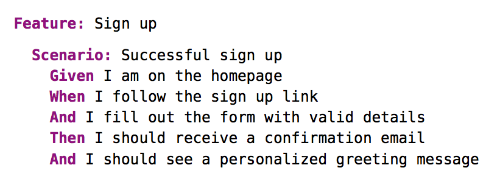
\includegraphics[width=0.8\textwidth]{codigo_cucumber}
    \caption{Um exemplo de código cucumber.}
    \label{fig:codigo_cucumber}
\end{figure}

\subsection{Selenium HQ}
É um \emph{framework} open source utilizado para automatização de testes funcionais em aplicações web \cite{chiavegatto1desenvolvimento}. Segundo \citeauthor{pereiraestudoselenium} \cite{pereiraestudoselenium}, se trata
de uma ferramenta de fácil uso e eficiente para desenvolver casos de teste, permitindo os testes de aceitação ou funcional, regressão e de desempenho.
Selenium trabalha como um plugin do navegador Firefox, o mesmo traz muita praticidade pois permite que se possa capturar cliques e valores digitados transformando-os em um caso de teste. Ele é composto por
quatro ferramentas: Selenium IDE, Selenium Grid, Selenium RC e Selenium WebDrive.

A  utilização  de  comandos  no  Selenium  consiste  em  digitar  o  comando  seguido  de  dois parâmetros  tal  como  por  exemplo \emph{verifyText //div//a[2] Login}. Dependendo  do  comando,  os parâmetros
poderão ser opcionais, aliás, alguns comandos não necessitam de parâmetros para serem executados \cite{sixpenceautomatizaccao}.

Selenium foi escolhida como umas das ferramentas no desenvolvimento deste projeto pelo fato de ser um \emph{framework open source} que possui um vasto leque de ferramentas para testes de sistemas web. Outro fator
importante para sua escolha é a possibilidade de interação do Selenium HQ com o Cucumber. Ela se destaca entre as demais ferramentas gratuitas pelo fato de ser a mais completa, permitindo integração com
várias linguagens, outros \emph{frameworks}, além de suportar inúmeros navegadores e sistemas operacionais \cite{pereiraestudoselenium}.

\subsection{JUnit}
JUnit é uma ferramenta de apoio ao teste unitário, a qual auxilia desenvolvedores na automação dos testes e verificação dos resultados \cite{biasi2006geraccao}. A escolha desta ferramenta, como parte integrante da solução desenvolvida deveu-se ao fato
de a mesma ser voltada para sistemas desenvolvidos na linguagem de programção Java, além de ser altamente versátil, possibilitando assim, integração em um único código da mesma com os demais \emph{frameworks} que seroã utilizados(Selenium e Cucumber).

Se justifica a sua utilização neste trabalho, por tratar-se de uma API (\emph{Application Programming Interface}) que viabiliza a comparação de um valor obtido em algum teste com o valor esperado pelo mesmo. Desta forma, pode-se validar e verificar se
a funcionalidade de um sistema está trabalhando adequadamente.

\section{Reuso de testes}

Visando melhor aproveitar os recursos existentes em uma instituição e ainda assim apresentar garantias na qualidade do produto/serviço entregues aos clientes, desenvolvedores do mundo todo, começaram a apresentar
teses e modelos que buscam criar testes genéricos e padronizados. Um padrão é um pedaço de informação instrutiva e nomeada, que captura a estrutura essencial
e \emph{“insights”} de uma família bem sucedida de soluções aprovadas para um determinado problema, o qual surge em um determinado contexto \cite{cagnin2004reuso}.

\citeauthor{guizzardi2000desenvolvimento} diz que por razões histórias a área de desenvolvimento de software não atingiu a maturidade que outras áreas da engenharia atingiram, complementa afirmando,
que apesar disso, é inegável que algum avanço tenha sido alcançado, pois a forma de realização dessa atividade evoluiu de uma atividade realizada de forma quase artesanal, para um processo de
desenvolvimento bem estruturado e que, nos melhores casos, contempla inclusive atividades de gerência e avaliação da qualidade \cite{guizzardi2000desenvolvimento}.
Com isso, a reutilização dos testes já codificados, se mostra uma importante prática no desenvolvimento e que ainda apresenta muitas incógnitas e possibilidades para as equipes de TI,
principalmente na geração de casos de testes que possam ser reutilizados em situações que apresentem um padrão parecido com os casos já conhecidos.

\chapter{Desenvolvimento}

Abaixo, serão descritas as atividades desenvolvidas a fim de alcançar os objetivos propostos por este trabalho. Será apresentada a estrutura básica dos sistemas escolhidos para inserção dos testes automatizados,
assim como trechos dos códigos desenvolvidos e estrutura das soluções encontradas ao longo do desenvolvimento do projeto.

\section{Delimitação de escopo}

Como escopo, foram delimitados alguns pré-requisitos necessários para utilização da solução proposta neste trabalho, onde, o sistema deve ser um software web, desenvolvido na linguagem de programação Java,
podendo apresentar também funções Ajax e Javascript.

\section{Visão geral da solução}
Em um primeiro momento, com objetivo de automatizar os testes de uma aplicação afim de reduzir o esforço na confecção e codificação de novos testes para as equipes de desenvolvimento e testes de uma empresa,
escolheu-se desenvolver uma solução baseada em três etapas que são descritas conforme imagem \ref{fig:solucao1}.

\begin{figure}[!htb]
	\centering
	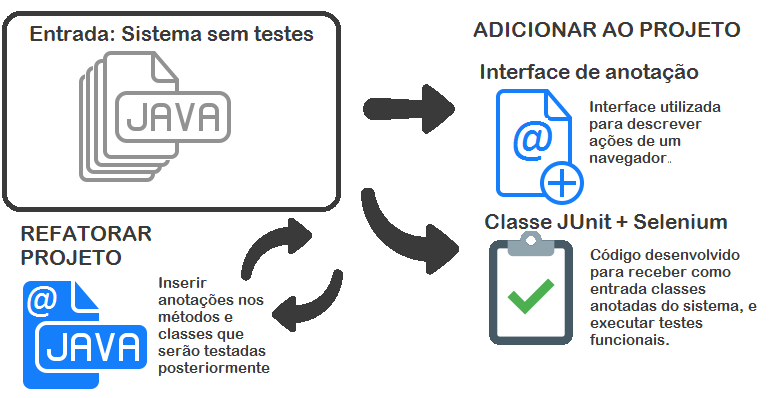
\includegraphics[width=0.8\textwidth]{solucao1}
	\caption{Estrutura da solução.}
	\label{fig:solucao1}
\end{figure}

Temos como ponto de partida um sistema onde se possui pouco ou nenhum teste codificado. Para o mesmo, descrevemos  três fases no desenvolvimento de uma solução em forma de testes para o sistema,
que seriam: criar uma classe de testes genérica, responsável por realizar os testes necessários na aplicação, descrever uma interface de anotação que representaria ações de elementos web (\emph{HTML}) que
seriam testados posteriormente e por fim inserir as anotações nos métodos e classes do sistema que devem ser testados nesta aplicação.

\section{Classe genérica de testes}
Por tratar-se de uma abordagem para sistemas web, optou-se pela utilização de dois frameworks de testes que possibilitam interações com elementos web para confecção da classe responsável pela execução dos testes automatizados,
o primeiro seria o Selenium. Através da utilização da classe \texttt{WebDrive}, contida no pacote do mesmo, podemos descrever uma sequência de passos que são executados por um navegador, como cliques e inserção de dados em campos de um
formulário. Sendo assim instanciando um objeto \texttt{WebDrive} podemos iniciar um navegador e realizar uma série de instruções pré-determinadas para validar se a aplicação comporta-se de forma adequada.

Por fim, necessitamos validar se após realizar o preenchimento de formulários do software, o resultado obtido condiz com o resultado esperado. Neste momento é onde se faz necessário a adição de trechos de códigos Junit na classe de teste
desenvolvida, pois o mesmo disponibiliza em seu pacote, um conjunto de métodos \emph{assert}, com os quais, se faz possível comparar, por exemplo, se após salvar um formulário de cadastro, a mensagem de "cadastrado com sucesso" aparece na tela.
A imagem \ref{code:TestaFormularios.java}, apresenta um trecho da classe confeccionada para realização dos testes.

\begin{figure}[!htb]
\begin{lstlisting}
@Test
public void testaFormularios() {
	for (Class classe : getCarregaClasses()) {
    		Teste testeClasse = TestePropriedades.teste(classe);
        if (testeClasse.fazerLogin()) {
            LoginTeste.login(TestePropriedades.urlSistema, testeClasse.getSenha(), testeClasse.getLogin(), webDriver);
        }
        if (!testeClasse.getUrl().equals("")) {
            webDriver.get(TestePropriedades.urlSistema + testeClasse.getUrl());
        }
        for(Method metodo: classe.getDeclaredMethods()) {
            Teste teste = TestePropriedades.teste(metodo);
            if (teste != null) {
                executaTeste(teste, true);
            }
        }
        executaTeste(testeClasse, false);
        System.out.println("Formulário da classe " + classe.getName() + " testado!");
	}
}
\end{lstlisting}
	\label{code:TestaFormularios.java}
\end{figure}

A classe desenvolvida possui um método principal denominado \texttt{testaFormularios}, onde a ideia principal do mesmo seria buscar
de forma recursiva, todas as classes do projeto anotadas pela interface que indica que a classe deve ser testada, e para cada uma das mesmas cria-se elementos \texttt{webDrive} para executar as ações indicadas pela anotação.

\section{Interface de anotação}

Após finalizar o desenvolvimento da classe de testes genérica, passou-se a existir a necessidade de criar um mecanismo para informar para a classe de testes, qual seriam as validações necessárias. Para esta tarefa,
por tratar-se de projetos Java, resolveu-se criar uma interface de anotação que seria vinculada aos métodos e classes onde, seriam necessários executar os testes posteriores. Desta forma, a classe \texttt{TestaFormulario.java},
responsável pela execução dos testes varreria as classes do sistemas e toda vez que encontra-se uma classe anotada por essa interface, executaria um teste, onde cada método que necessitaria de um teste possuiria em sua anotação o tipo do campo,
as ações que deveriam ser executas e o valor que deveria ser preenchido.

Deu-se o nome de \texttt{Teste.java} para a interface, e sua estrutura está ilustrada em \ref{code:Teste.java}.

\begin{figure}[!htt]
\begin{lstlisting}
@Documented
@Retention(RetentionPolicy.RUNTIME)
@Target({ElementType.TYPE, ElementType.METHOD})
public @interface Teste {
    String getUrl() default "";

    //findElement
    String getCampo() default ""; //campo html do formulário
    String getIdentificador() default "id"; //Informar se deve buscar um id, name, class ou css

    boolean isSelect() default false;

    String getValor() default ""; //utilizado como sendKeys e selectText
    boolean click() default false;
    boolean submit() default false;
    boolean limpar() default false;

    String getTipoAssert() default "igual";
    String getCampoAssert() default "";
    String getIdentificadorAssert() default "id";
    String getValorEsperadoAssert() default "";
    String getAtributoCampoComparacaoAssert() default "texto";

    boolean fazerLogin() default false;
    String getLogin() default "colegiado";
    String getSenha()default "";
}
\end{lstlisting}
	\caption{Interface Teste}
	\label{code:Teste.java}
\end{figure}

Tem-se então que cada método existente nesta classe representa uma ação específica da classe \texttt{WebDrive}, possibilitando assim manipular elementos \emph{HTML} na execução do teste.

\section{Inserção das anotações no projeto}
Por fim, a ultima etapa da solução em questão, trata-se de uma etapa contínua no projeto, pois sempre que uma nova classe é mapeada no sistema ou um novo cadastro é criado, a mesma ocorrerá. Nesta etapa se faz necessário a
adição das anotações nos códigos do projeto, onde se deve inserir a anotação em todas as classes e métodos que devem ser testados.
A \ref{code:Disciplina.java} ilustra e exemplifica a forma como ocorre as anotações utilizando a interface Teste em uma determinada classe Java.

\begin{figure}[!htt]
\begin{lstlisting}
@Teste(getUrl = "/cadastro-disciplina.htm", getCampo = "salvar", click = true,getIdentificadorAssert = TestePropriedades.IDENTIFICADOR_CSS, getCampoAssert = "h4", getValorEsperadoAssert = "Sucesso!")
public class Disciplina {
    private String codigo;
    private String nome;
    private Integer cargaHoraria;

    @Teste(getCampo = "ativa1", click = true)
    public Boolean getAtiva() {
        return ativa == null || ativa;
    }

    public void setAtiva(Boolean ativa) {
        this.ativa = ativa;
    }

    @Teste(getCampo = "cargaHoraria", getValor = "60", isSelect = true)
    public Integer getCargaHoraria() {
        return cargaHoraria;
    }

    public void setCargaHoraria(Integer cargaHoraria) {
        this.cargaHoraria = cargaHoraria;
    }

    @Teste(getCampo = "nome", getValor = "Disciplina teste")
    public String getNome() {
        return nome;
    }
}
\end{lstlisting}
	\caption{Classe anotada com @Teste}
	\label{code:Disciplina.java}
\end{figure}

Na anotação são inseridas informações referente as ações que devem ser executadas para a propriedade em questão. Os métodos possuem anotações referentes apenas ao campo que representam, enquanto as informações mais gerais sobre
a página que está sendo testada, são inseridas na anotação da Classe propriamente dita.

\section{Discussão sobre a solução}
Após a finalização do desenvolvimento desta primeira solução encontrada, notou-se a clara necessidade de alteração na sistemática de como os teste ocorreriam, necessidade esta oriunda de algumas limitações que a solução trás,
como por exemplo, a não possibilidade de realizar testes que envolvam mais de um método, tornando praticamente inviável a tarefa de realizar testes funcionais, pois não seria possível mapear um cenário mais completo, que depende
de mais de uma variável e que tem uma sequência bem mapeada que deve ser seguida.

Outro fator determinante paraa alteração desta solução, foi o fato de por utilizar anotações, o mesmo não possibilitaria o teste de um mesmo campo, com dois valores diferentes, pois só seria possível informar na anotação do
método um valor de teste. Além disto, também não seria viável a execução de testes unitários para um sistema muito grande, pois é sabido que os testes devem ser executados sobre os pontos críticos do software e não na totalidade do projeto.

\chapter{Próximas Etapas}
Como continuação do trabalho realizado até o momento, são planejadas as seguintes atividades:

\begin{enumerate}
	\item Alterar a modelagem visando permitir a realização de testes funcionais: Para permitir que cenários sejam contemplados por testes funcionais, será
	acoplado a solução a utilização da linguagem Cucumber, onde cada cenário sera descrito por um conjunto de ações do Selenium.
	\item Ampliar área de abrangência da solução: Implementar e disponibilizar suporte para elementos mais complexos.
	\item Realizar comparações para validar solução genérica desenvolvida: Apresentar motivos pelo qual deve-se utilizar a solução e o ganho que a mesma trás para uma equipe que possui
	recursos humanos limitado.
\end{enumerate}

\setlength{\baselineskip}{\baselineskip}
\bibliographystyle{abnt}
\bibliography{../referências}
\end{document}
